% @CTB read CAMI

%
% - Are plasmids present in the reference dataset?
% - Reformat column tables for readability
% - Add carbon footprint to assembly stats  

%%%%%%%%%%%%%%%%%%%%%%%%%%%%%%%%%%%%%%%%%%%%%%%%%%%%%%%%%%%%%%%
%
% Welcome to Overleaf --- just edit your article on the left,
% and we'll compile it for you on the right. If you give 
% someone the link to this page, they can edit at the same
% time. See the help menu above for more info. Enjoy!
%
%%%%%%%%%%%%%%%%%%%%%%%%%%%%%%%%%%%%%%%%%%%%%%%%%%%%%%%%%%%%%%%
%
% For more detailed article preparation guidelines, please see:
% http://f1000research.com/author-guidelines

\documentclass[10pt,a4paper,twocolumn]{article}
\usepackage{f1000_styles}
\usepackage{multirow} 
%% Default: numerical citations
\usepackage[numbers]{natbib}

\setlength{\parskip}{0.2em}

%% Uncomment this lines for superscript citations instead
% \usepackage[super]{natbib}

%% Uncomment these lines for author-year citations instead
% \usepackage[round]{natbib}
% \let\cite\citep

\begin{document}

\title{\textit{F1000Research} Evaluating Metagenome Assembly on a Complex Community}
\titlenote{ }
\author[1]{Sherine Awad}
\author[2]{Luiz Irber}
\author[3]{C. Titus Brown}
\affil[1,2,3]{Department of Population Health and Reproduction, University of California, Davis, California}
 

\maketitle
\thispagestyle{fancy}

% Please list all authors that played a significant role in the research involved in the article. Please provide full affiliation information (including full institutional address, ZIP code and e-mail address) for all authors, and identify who is/are the corresponding author(s).

\begin{abstract}
 

 
Metagenome assembly is a challenging problem due to the biodiversity
of the microorganisms. Most assemblers are designed for whole genome
assembly and not capable of dealing with metagenomic samples. However,
in order to decide which assembler works best for metagenome, we need
to evaluate metagenome assembly generated by each assembler.

% CTB: mention microdiversity, species foo.

In this paper, we used three assemblers ; IDBA-UD, SPAdes, and Megahit
to assemble metagenome mock community data and evaluate the assembly
process in terms of resources utilization, assembly quality, genome
fraction covered, duplication ratio, misassemblies and partial
alignments.

The results show only small differences in content recovery between
assemblers. However, Megahit is much faster and produces shorter
contig lengths than IDBA-UD and SPAdes.
 


%Motivation: With the emergence of de novo assembly, several work have been done to assemble metagenomic data from de novo. Several assemblers exist that are based on different assembly techniques. However, we still lack  a study that analyze different assemblers behaviors on metagenomic data. 
 
%Problem statement: In this paper, we performed an analytic study for metagenome assembly using different assemblers. The aim of the analysis is studying how well metagenome assembly works, and which assembly works best.  


%Approach: We used a mock community dataset for the analysis, and used its reference genome for the benchmark evaluation. We quality filtered the reads  then assembled the reads using three different assemblers: IDBA-UD, SPAdes, and MEGAHIT.


 

\end{abstract}

\clearpage

\section*{Introduction}

Metagenomics refers to sequencing of DNA from a mixture of organisms,
often from an environmental or uncultured sample. Unlike whole genome
sequencing, metagenomics targets a mixture of genomes, which
introduces metagenome-specific challenges in analysis.  Most
approaches to analyzing metagenomic data rely on mapping or comparing
sequencing reads to reference sequence collections. However, reference
databases contain only a small subset of microbial diversity (cite:
geba), and the much of the remaining diversity is evolutionarily distant
and search techniques may not access it.

As sequencing capacity increases and sequence data is generated from
many more environmental samples, metagenomics is increasingly using de
novo assembly techniques to generate new reference genomes and
metagenomes.  There are a number of metagenome assemblers that are
widely used. However, evaluating the results of these assemblers is
challenging due to the general lack of good quality reference
metagenomes.  Below, we evaluate three commonly assemblers - SPAdes,
IDBA, and MEGAHIT - on a mock community containing 64 species of
microbes with known genomes.

% @CTB reference megahit 1.0 paper which did an assembly and evaluation
% of the same data set as us.

 
%-----------Literature Review starts here ---------------------

% @CTB do a few quick checks, but I don't know of any benchmark studies
% other than these.
 
Moya et al. in \cite{moya2014} evaluated metagenome assembly using
two simulated 454 viral metagenome and six assemblers. The assemblies
were evaluated based on several metrics including N50, percentages of
reads assembled, accuracy when compared to the reference genome. In
addition to, chimeras per contigs and the effect of assembly on
taxonomic and functional annotations.
 
Mavromatis et al. in \cite{mavromatis2007} provided a benchmark study
to evaluate the fidelity of metagenome process methods. The study used
simulated metagenomic data sets constructed at different complexity
levels.
%The low complexity set is dominated by a single near-clonal organism. The medium complexity set includes moderate communities with more than one dominant organism. The high complexity set lacks dominant population.  
The datasets were assembled using Phrap v3.57, Arachne v.2
\cite{arachne} and JAZZ. \cite{jazz}
This study evaluates assembly, gene prediction, and binning
methods. However, the study did not evaluate the assembly quality
against a reference genome.

Rangwala et al. in \cite{huzefa2011} presented an evaluation study of
metagenome assembly. The study used a de Bruijn graph based assembler
ABYSS \cite{abyss} to assemble simulated metagnome reads of 36 bp. The
data set is classified at different complexity levels.
%The data set is classified into 3 classes, low complexity data set in which the reads belongs to a single dominant organism, a medium complexity data set, in which the reads has more than one dominant organism with lower concentration, and the high complexity data set which has no distinct dominant organism.
The study compares the quality of the assembly of the data sets in
terms of quality measures of contigs length, assembly accuracy. The
study also took into consideration the effect of kmer size and the
degree of chimericity.  However, the study evaluated the assembly
based on one assembler, and did not evaluate assembly against several
assemblers.  Also, both previous studies used simulated data, which
may lack confounders of assembly such as sequencing artifacts and GC bias.

Shakya et al. (2013) constructed a complex synthetic community of
organisms by mixing DNA isolated from individual cultures of 64
bacteria and archaea.  In addition to performing 16s amplicon analysis
and doing 454 sequencing, the authors shotgun sequenced the mixture
with Illumina (@cite).  While the authors concluded that this metagenomic
sequencing generally outperformed amplicon sequencing, they conducted
a mapping based analysis rather than an assembly based analysis.

% @CTB pignatelli & moya 2011

More recently, several benchmark studies systematically evaluated
metagenome assembly of short reads. (CAMI and ...)

In this paper, we evaluate metagenome assembly on the Illumina data set from
Shakya et al. (2013) using three assemblers; IDBA-UD \cite{idba},
SPAdes \cite {spades}, and MEGAHIT \cite{megahit}.  These three assemblers
were chosen because they are actively used and highly cited.

SPAdes \cite{spades} is an assembler for both single-cell and standard
(multicell) assembly. (More description here @CTB.)

IDBA-UD \cite{idba} is a de Bruijn graph
approach for assembling reads from single cell sequencing or
metagenomic sequencing technologies with uneven sequencing
depths. IDBA-UD uses multiple depth-relative thresholds to remove
erroneous k-mers in both low-depth and high-depth regions. It also
uses paired-end information to solve the branch problem of low-depth
short repeat regions. It also applies an error correction step to correct
reads of high-depth regions that can be aligned to high confident
contigs.

MEGAHIT \cite{megahit} is a newer approach that constructs a succinct
de Bruijn graph using multiple k-mer sizes, and uses a novel ``mercy
k-mer'' approach that preserves low-abundance regions of reads. It also
can use GPUs to accelerate the graph construction.

Below, we evaluate the performance of these three assemblers using the
synthetic (``mock'') community data from the Shakya et al. study.
The performance of each assembler is compared in terms
of resource utilization, covered genome fraction, duplication ratio, gene
recovery, contig misassembly, and contig length.

In contrast to some other evaluations (assemblathon 2), we work with a
synthetic community with a known answer, do not tune the default
parameters, and investigate memory and runtime as a key part of the
process.  This mimics default user experience. (Expand.)

In this report, we update the list of reference genomes for Shakya et
al.  to include plasmids and compare IDBA, SPAdes, and MEGAHIT
performance on short-read metagenome assembly.  We also evaluate
inter-strain chimerism in the assemblies, explore the failure to
recover a specific {\em Shewanella baltica} strain variant in the
assembly, and detect several previously unreported genomes in the
Shakya et al. data set.  Our report provides strong guidance on choice
of assemblers and significantly extends previous analyses of this
low-complexity metagenome benchmarking data set.

% \subsection*{Sections}

% Use section and subsection commands to organize your document. \LaTeX{} handles all the formatting and numbering automatically. Use ref and label commands for cross-references.


% Removed this line for now \subsection*{Tables}

% Use the table and tabledata commands for basic tables --- see Table~\ref{tab:widgets}, for example.
% \begin{table}[h!]
% \hrule \vspace{0.1cm}
% \caption{\label{tab:widgets}An example of a simple table with caption.}
% \centering
% \begin{tabledata}{llr} 
% \header First name & Last Name & Grade \\ 
% \row John & Doe & $7.5$ \\ 
% \row Richard & Miles & $2$ \\ 
% \end{tabledata}
% \end{table}
 
%-----------------------------Misassembles table 

 
\begin{figure}[!h]
\centering
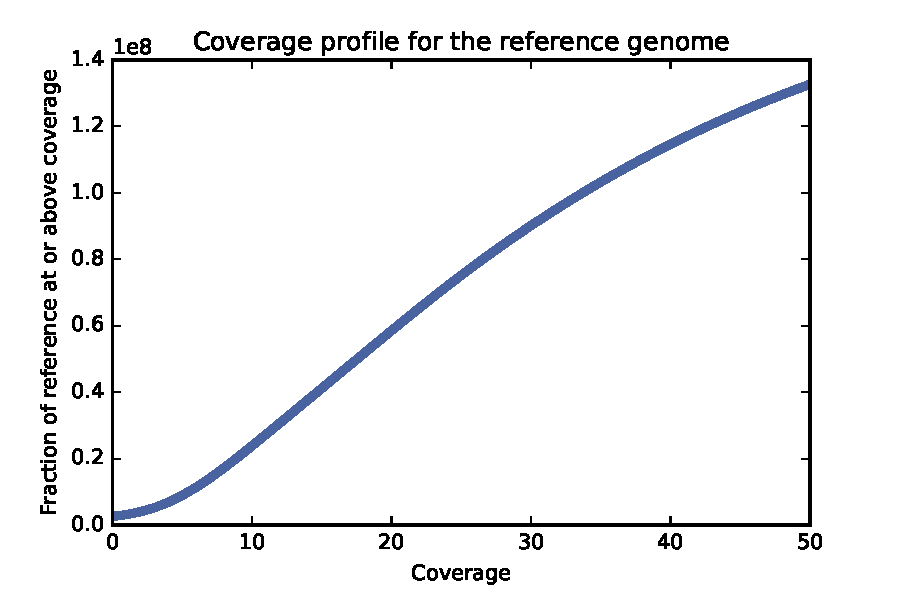
\includegraphics[width=0.45\textwidth]{CoverageProfile.pdf}  
\caption{\label{fig:coverage-profile} Cumulative coverage profile for the reference metagenome, based on read mapping. }
\end{figure}

%\begin{figure}[!h]
%\centering
%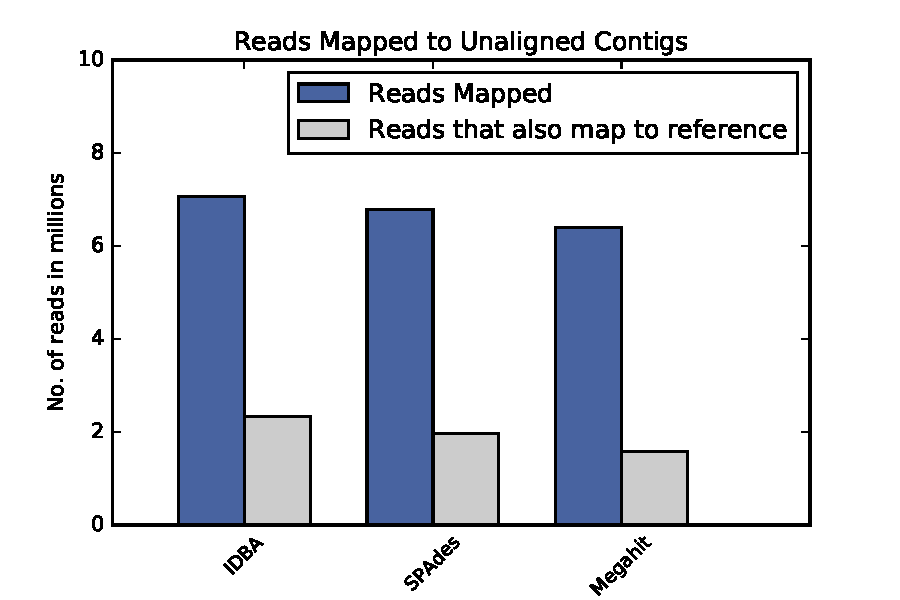
\includegraphics[width=0.45\textwidth]{UnalignmentHistogram.pdf} %to be chamged to qc.coverage-profile
%\caption{Mapping unaligned reads to reference genome using identity 99\%, and Ambiguous Approach CTB This can't be right :)}
%\label{fig:unaligned-reads}
%\end{figure}

% \begin{figure}[!ht]
% \centering
% 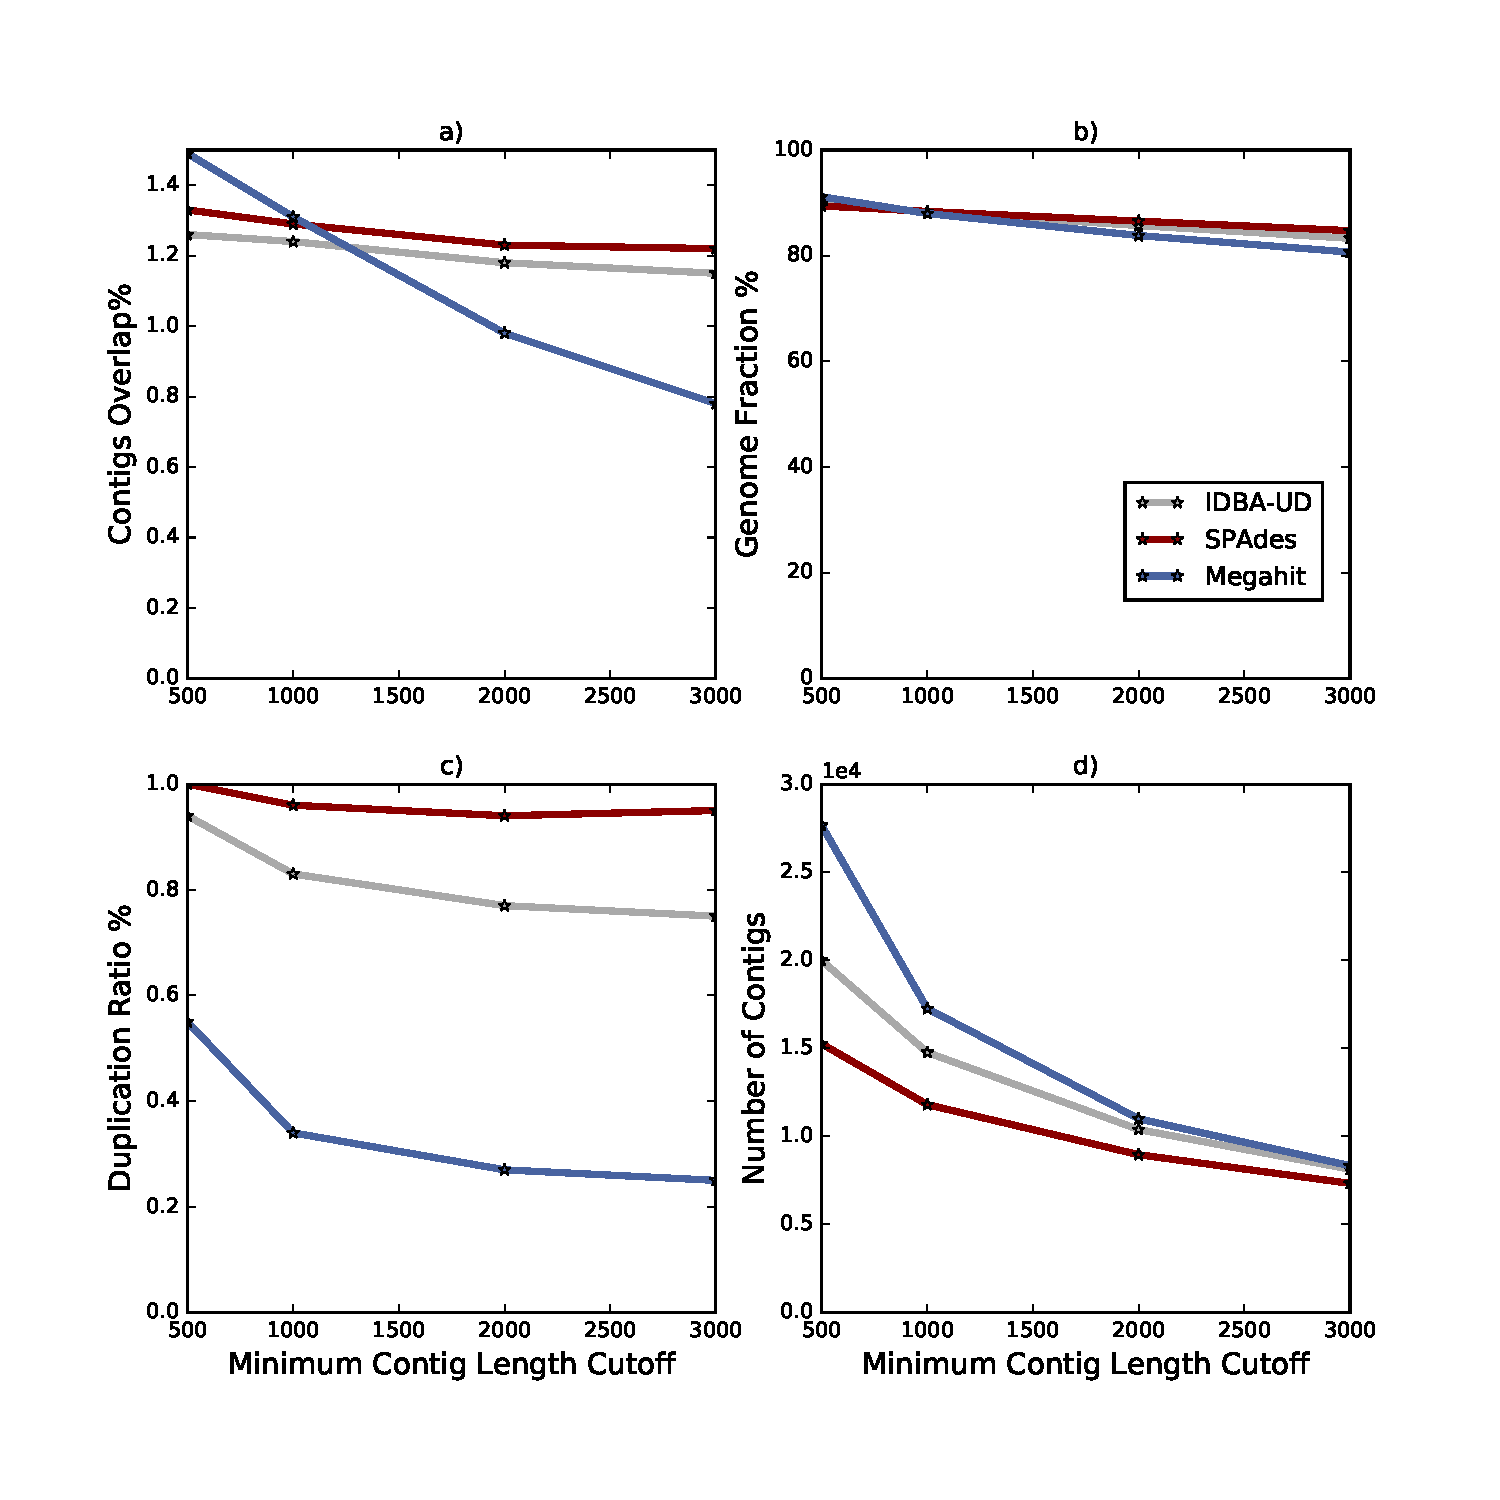
\includegraphics[width=9.5cm,height=9.5cm]{min-contig-analysis.pdf}  
% \caption{\label{fig:min-contig-analysis} Genome fraction, duplication ratio, Contigs overlap ratio, and number of contigs using different minimum contig length,  identity 99\%, and Ambiguous Approach}
% \end{figure}

% @CTB maybe we should put this back in?
% \begin{figure}[!h]
% \centering
% 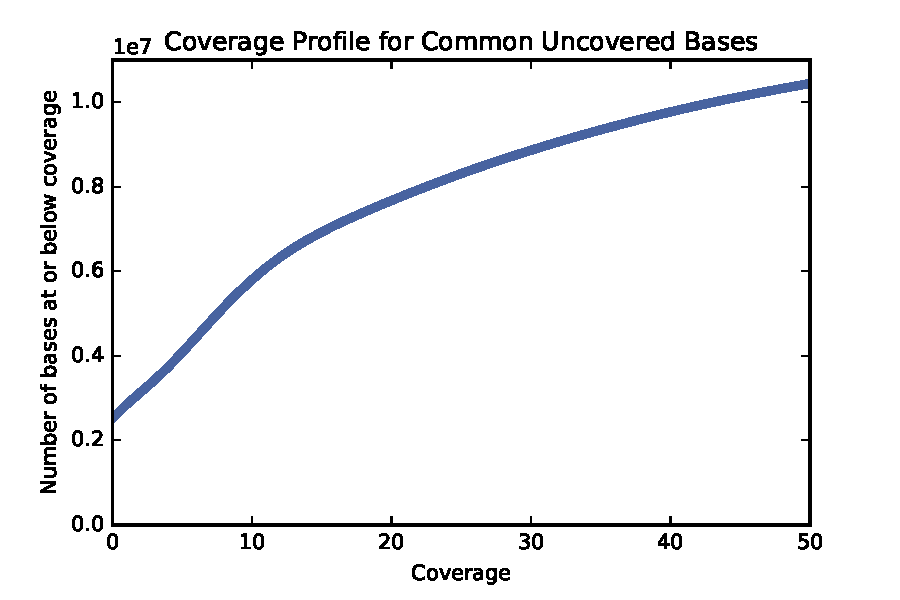
\includegraphics[width=0.4\textwidth]{CommonUncoveredCoverageProfile.pdf} 
% \caption{Cumulative read coverage for bases in the reference metagenome missing from all three assemblies.}
% \label{fig:CommonUncovered}
% \end{figure}



% \begin{figure}[!h]
% \centering
% \includegraphics[width=0.4\textwidth]{MapQuality.png}  
% \caption{\label{fig:mapquality} Mapping Quality for Quality Filtered Reads to the Reference Genome}
% \end{figure}

% \begin{figure}[!h]
% \centering
% \includegraphics[height=2.6cm,width=0.4\textwidth]{basequality.png}  
% \caption{\label{fig:basequality} Mean Base Quality}
% \end{figure}

% \begin{figure}[!h]
% \centering
% \includegraphics[height=2.6cm, width=0.4\textwidth]{errorprofile30.png}  
% \caption{\label{fig:errorprofile30}Error Profiles for MAPQ >=30}
% \end{figure}

% \begin{figure}[!h]
% \centering
% \includegraphics[height=2.6cm, width=0.4\textwidth]{nucleotidecomposition.png}  
% \caption{\label{fig:nucleotidecomposition.png}Nucleotide Composition for MAPQ >=30}
% \end{figure}
% \subsection*{Mathematics}

 
% \subsection*{Mathematics}

\subsection*{Datasets}
%Numbers in this section are up to date 22 december 2016

We used a diverse mock community data set constructed by pooling DNA
from 64 species of bacteria and archaea and sequencing them with
Illumina HiSeq.  The raw data set consisted of 109,629,496 reads from
Illumina HiSeq 101 bp paired-end sequencing (2x101) with an untrimmed
total length of 11.07 Gbp and an estimated fragment size of 380 bp
\cite{podar}.
 
The original reads are available through the NCBI Sequence Read
Archive at Accession SRX200676.
We received the 64 reference genomes from the original authors. They
consist of 205.6 Mbp of assembled genomes in 64 contigs, and are
available for download at
https://dx.doi.org/10.6084/m9.figshare.1506873.v2.

We updated the data sets from NCBI etc. etc.  The following genomes
were updated.  Updated data is available for download here (OSF).

\section*{Methods}
The analysis code and run scripts for this paper are available at:
https://github.com/dib-lab/2015-metagenome-assembly/. The scripts and
overall pipeline were examined by the first and senior authors for
correctness.  In addition, the bespoke reference-based analysis
scripts were tested by running them on a single-colony {\em E. coli} MG1655
data set with a high quality reference genome \cite{chitsaz2011}.

\subsection*{Quality Filtering} 

We removed adapters with Trimmomatic v0.30 in paired-end mode with the
Truseq adapters \cite{trimmomatic}, using light quality score trimming
as recommended in MacManes, 2014 \cite{macmanes2014optimal}.

%We next used the fastq\_quality\_filter from the FASTX-Toolkit v0.0.13.2  \cite{FXtoolkit} to remove sequences using the parameters  {\tt{-Q33   -q 30 --p 50}} , which keeps all sequences with  50\%  or more bases with quality score greater than or equal to 30.

\subsection*{Reference Coverage Profile}

To evaluate how much of the reference metagenome was contained in the read
data, we used {\tt bwa aln} to map reads to the reference genome.  We then
calculated how many reference bases were covered by how many mapped
reads (custom script {\tt coverage-profile.py}).

\subsection*{Assemblers}
We assembled the quality-filtered reads using three different assemblers: IDBA-UD
\cite{idba}, MetaSPAdes \cite{spades}, and MEGAHIT \cite{megahit}.  For
IDBA-UD v1.1.1 \cite{idba}, we used {\tt {--pre\_correction}} to
perform pre-correction before assembly and -r for the pe files.

For MetaSPAdes v3.9.0 \cite{spades}, we used { \tt {--meta --pe1-12
    --pe1-s}} where {\tt{--meta}} is used for
metagenomic data sets, {\tt{--pe1-12}} specifies the interlaced reads
for the first paired-end library, and {\tt{--pe1-s}} provides the
orphan reads remaining from quality trimming.

For MEGAHIT v1.1.1-2-g02102e1 \cite{megahit}, we used -l 101 {\tt{-m 3e9
    --cpu-only}} where {\tt -l} is for maximum read length, {\tt -m} is
for max memory in bytes to be used in constructing the graph, and {\tt
  {--cpu-only}} to use only the CPU and no GPUs. We also used {\tt
  {--presets meta-large}} for large and complex metagenomes, and {\tt
  {--12} } and {\tt{-r}} to specify the
interleaved-paired-end and single-end files respectively.  MEGAHIT allows
the specification of a memory limit and we used {\tt -M 1e+10} for 10 GB.

All three assemblies were executed on the same high-memory buy-in node
on the Michigan State University High Performance Compute Cluster, and
we recorded RAM and CPU time of each assembly job using the {\tt
  qstat} utility at the end of each run.

Unless otherwise mentioned, we eliminated all contigs less than 500 bp
from each assembly prior to further analysis.

\subsection*{Mapping}

We aligned all quality-filtered reads to the reference metagenome with
bwa aln (v0.7.7.r441) \cite{bwa}. We aligned paired-end and orphaned
reads separately. We then used samtools (v0.1.19)
\cite{sam-stools} to convert SAM files to BAM files for both
paired-end and orphaned reads. To count the unaligned reads, we
included only those records with the ``4'' flag in the SAM files
\cite{sam-stools}.
 

To extract the reads that contribute to unaligned contigs, we mapped
the quality filtered reads to the unaligned contigs using bwa aln
(v0.7.7.r441) \cite{bwa}.  Then we used samtools to retrieve the reads
that mapped to the unaligned contigs.


%We found chimeric alignments (alignments that split reads in two or more) with the bwa mem aligner using the default parameters (v0.7.7.r441). 

%To count the chimeric alignments, we count the secondary alignments (records with the ``SA" flag) in the SAM file \cite{samtools}. 

%We used SamStats \cite{samstats} to analyze the quality of mapping and errors. 

\subsection*{k-mer Presence}
In order to examine k-mer presence for a k-mer size of 20, we built a
k-mer counting table from the given quality filtered reads using
{\tt{load-into-counting.py}} from khmer \cite{khmer2016}. Then we
calculate abundance distribution of the k-mers in the quality filtered
reads using the pre-made k-mer counting table using
{\tt{abundance-dist.py}}. We followed the same approach to examine
k-mer presence in assemblies.

\subsection*{Assembly analysis using Nucmer}

We used the NUCmer tool from MUMmer3.23 \cite{mummer3.0} to align
assemblies to the reference genome with options {\tt \--coords} {\tt
  -p}. Then we parsed the generated ``.coords'' file using a custom
script {\tt{analyze\_assembly.py}}, and calculated several analysis
metrics across all three assemblies at two alignment identities, 95\% and 99\%.

\subsection*{Reference-based analysis of the assemblies}

We analyzed metrics for three different sets of contigs, based on the
NUCmer alignments.  We used the unfiltered NUCmer alignments for the
analyses termed ``ambiguous.''  We also subjected the alignments to
two different filtering criteria, ``best-hit'' and
``no-misassemblies.''
In the best-hit approach, among all alignments of a contig, we took
into consideration the longest alignment with an identity above a specified
identity threshold (either 95\% or 99\%).
In the no-misassemblies approach, we only counted contigs that have
precisely one alignment within the reference.

In all approaches, we flag a base in the reference genome as
``covered'' if it is contained in a kept alignment.  We define the
duplication ratio as the percentages of bases in the reference covered
by two or more kept alignments. We define misassemblies as
those contigs that are divided into different parts when mapped to the
reference.  The number of misassembled contigs is equal to the number
of aligned contigs (both totally and partially) in the ambiguous
approach, minus the number of aligned contigs in the no-misassemblies
approach.

%We define the contig overlap ratio as the number of bases
%aligned to the reference that exist in more than one contig.  We
%define the contig overlap ratio as the number of bases aligned to the
%reference that exist in more than one kept alignment.

All approaches have a non-zero duplication ratio within the reference
because we do not explicitly discard contigs that map to the same
location in the reference.

\subsection*{Analysis of chimeric misassemblies}

%@CTB cami, disco just used quast.

We analyzed each assembly for chimeric misassemblies by counting the
number of contigs that contained matches to two distinct reference
genomes.  In order to remove secondary alignments from consideration,
we first filtered matches extracted the longest non-overlapping NUCmer
alignments for each contig at a minimum alignment identity of 99\%.
We then used the script {\tt analyze\_chimeric2.py} to find contigs
that matched sequences two or more distinct reference species.  As a
negative control on our analysis, we verified that this approach
yielded no positive results when applied to the alignments of the
reference metagenome against itself.

%@CTB Note: The rate of chimerism is probably higher when you include Shewanella OS185 and bordetella and haloferax.
% @CTB note that cami reported megahit has highest # misassemblies.


%\subsection*{Gene annotations using Prokka}
%We used prokka \cite{prokka} to annotate the reference genome using
%{\tt{--metagenome}}. Then we parsed
%the testasm.tbl output file to get the coordinates of CDS genes and
%searched the alignments for how many genes were contained in those
%alignments.
% @CTB what script?

\section*{Results}

\subsection*{The raw data is high quality.}

The reads contains 11,072,579,096 bp (11.07 Gbp) in 109,629,496 reads
with 101.0 average length (2x101bp Illumina HiSeq).

Trimming removed 686,735 reads (0.63\%).  After trimming, we retained
108,422,358 paired reads containing 10.94 Gbp with an average length of
100.9 bases. A total of 46.56 Mbp remained in 520,403 orphan reads with
an average length of 89.5 bases. In total, the quality trimmed data
contained 10.98 Gbp in 108,942,761 reads.  This quality trimmed ("QC")
data set was used as the basis for all further analyses.
% These numbers are calculated using readstats from khmer

%\subsection*{Mapping Quality and Error Profiles}

%%Might need to be merged with previous section  @CTB
%We used SAMStat \cite{samstat} to analyze the mapping quality and error profiles of quality filtered reads mapped to the reference genome. Figure \ref{fig:mapquality} shows number of alignments in various mapping quality (MAPQ) intervals and number of unmapped sequences. The percentage and number of alignments in each category is given in brackets. 
%Figure \ref{fig:basequality} shows mean base quality of reads with low and high mapping quality. %Figure \ref{fig:errorprofile30} shows the error profile for MAPQ $\geq 30$ and Figure \ref{fig:nucleotidecomposition.png} shows the nucleotide compositions. We also found 309,414 chimeric reads. 

\subsection*{The reference metagenome is not completely present in the reads.}

We next evaluated the fraction of the reference genome covered by at least
one read (see Methods for details). Quality filtered reads cover
203,058,414 (98.76\%) bases of the reference metagenome (205,603,715
bp total size).  Figure \ref{fig:coverage-profile} shows the
cumulative coverage profile of the reference metagenome, and the
percentage of bases with that coverage. Most of the reference
metagenome was covered at least minimally; only 3.33\% of the
reference metagenome had mapping coverage \textless 5, and 1.24\% of
the bases in the reference were not covered by any reads in the QC data
set.

\begin{table}[t]
\caption{Jaccard containment of the reference in the reads}
\centering
\begin{tabular}{|c|c|}
\hline
\textbf{k-mer size} & {\textbf \% reference in reads } \\ [0.5ex]
\hline
21 & 96.8\% \\
\hline
31 & 95.9\% \\
\hline
41 & 94.9\% \\
\hline
51 & 94.1\% \\
\hline
\end{tabular}
\label{table:ref_in_reads}
\end{table}

In order to evaluate reconstructability with De Bruijn graph
assemblers, we next examined k-mer containment of the reference in the
reads for $k$ of 21, 31, 41, and 51 (Table \ref{table:ref_in_reads}).
The k-mer overlap decreases from 96.8\% to 94.1\% as the k-mer size
increases. This could be caused by low coverage of some portions
of the reference and/or variation between the reads and the reference.


%Of
%the 174m 20-mers in the reference metagenome, 98.7\% were present in the
%QC reads and 95.5\% of them occurred with abundance 5 or greater in
%the QC reads.
%Data source note: the 95.5 is from
% SRR606249.qc.dist (1-0.045)*100 , the 98.7 is from the same file but
% (1-0.013) *100

\subsection*{Some individual reference genomes are poorly represented in the reads.}

% measured in *.cov.txt

\begin{table}[!h]
\centering
\caption{Top uncovered genomes}
\begin{tabular}{|l|c|c|}\hline
\textbf{Genome} & \textbf {Read coverage} & \textbf{21-mer presence} \\ \hline 
% 7.fa
{{\em B. xenovorans}} & 99.2\% & 91.6\% \\
\hline
% 17.fa
{{\em D. vulgaris} DP4}  & 91.98\% & 79.1\% \\
\hline
% 55
{{\em T. thermophilus} HB27}  & 91.06\% & 79.7\% \\
\hline
% 19
{{\em E. faecalis} V583}  & 78.14\% & 68.0\% \\
\hline
% 20
{{\em F. nucleatum}}  & 47.6\% & 17.8\% \\

% 18.fa.cov.txt:18.fa.cov.sam
{{\em }} & 89.22\& & XX\% \\
% 10.fa.cov.txt:10.fa.cov.sam
{{\em }} & 87.69\& & XX\% \\
% 11.fa.cov.txt:11.fa.cov.sam
{{\em }} & 85.16\& & XX\% \\
% 14.fa.cov.txt:14.fa.cov.sam
{{\em }} & 80.00\& & XX\% \\
% 15.fa.cov.txt:15.fa.cov.sam
{{\em }} & 79.07\& & XX\% \\
% 19.fa.cov.txt:19.fa.cov.sam
{{\em E. faecalis}} & 74.62\& & XX\% \\
% 17.fa.cov.txt:17.fa.cov.sam
{{\em D. vulgaris}} & 62.37\& & XX\% \\
% 19.fa.cov.txt:19.fa.cov.sam
{{\em E. faecalis}} & 61.86\& & XX\% \\
% 16.fa.cov.txt:16.fa.cov.sam
{{\em D. radiodurans}} & 55.33\& & XX\% \\
% 20.fa.cov.txt:20.fa.cov.sam
{{\em F. nucleatum }} & 47.58\& & XX\% \\


\hline
\end{tabular}
\label{table:genomes_uncovered-analysis}
\end{table}

% @CTB verify mqc 47.41 against Shewanella baltica.

% @ find/calculate read coverage for Burkholderia
% @ compare with estimates from shakya paper

To see if specific reference genomes exhibited low coverage, we
analyzed read mapping coverage and 21-mer containment for individual
genomes.  Of the 64 reference genomes used in the metagenome, 59 had a
per-base mapping coverage above 95\% and a 21-mer containment in the
QC reads above 95\%.  The remaining five varied significantly in both
metrics (Table~\ref{table:time-memory}), with {\em F. nucleatum} the
lowest -- only 47.30\% of the bases in the reference genome are
covered by one or more mapped reads, and only 17.8\% of the 21-mers in
the {\em F. nucleatum} reference genome are present in the reads at
any abundance.

% @CTB: point out in discussion that read mapping correlates well with
% k-mer presence.

We next did a 51-mer containment analysis of each reference genome in
the reads.  99\% or more of the constituent 51-mers for 51 of the 64
reference genomes were present in the reads, suggesting that each
of the 51 genome was entirely present at some minimal coverage.

We excluded the remaining 13 genomes from any comparative
analysis of assembly quality, because interpreting coverage and
misassembly analysis for these genomes would be impossible.
(@CTB list or table?)

% new reference size: 141,394,815

% @CTB: point out in discussion that whether low coverage or strain variation,
% not fair to analyze misassemblies when k-mers entirely absent.

\subsection*{MEGAHIT is the fastest and lowest-memory assembler evaluated}
%Numbers in this section are up to date 22 december 2016

 %------------------------------------Cost of Assembly ---------------
 \begin{table}[h]
\caption{Running Time and Memory Utilization}
\centering
\begin{tabular}{|l|c|c|c|}
\hline
\textbf{Assembler} & \textbf{CPU time} & \textbf{Wall time} & \textbf{RAM} \\ [0.5ex]
\hline
MEGAHIT & 52hr 25m & 4 hr 9m & 11.4 GB \\
\hline
IDBA-UD & 17h & & 149.1 GB \\
\hline
SPAdes & 94hr 43m & 94hr 44m & 100.7 GB \\
\hline

\end{tabular}
\label{table:time-memory}
\end{table}

 We ran three commonly used metagenome assemblers on the QC data set:
IDBA-UD, SPAdes, and MEGAHIT. We recorded the time and memory usage of
each (Table \ref{table:time-memory}).  In computational requirements, MEGAHIT outperformed both
SPAdes and IDBA-UD considerably, producing an assembly in four hours --
approximately 4 times faster than IDBA and 8 times faster than
SPAdes.  MEGAHIT used only 11.4 GB of RAM -- 1/13th to 1/9th
the memory used by IDBA and SPAdes, respectively.

% see pipeline/runtimes/

\subsection*{The assemblies contain most of the raw data}
%Numbers in this section are up to date 22 december 2016

%--------------------------Mapped reads and kmer abundance 


\begin{table}[!h]
\centering
\caption{Read and k-mer exclusion from assemblies}
\begin{tabular}{|p{1.5cm}|p{1.5cm}|p{2.5cm}|}\hline
  \textbf{Assembly} & \textbf{Unmapped Reads} & \textbf {51-mers omitted}
  \\ \hline
IDBA &3,328,674 (3.05\%)&  3.4\% \\ \hline
SPAdes &3,879,573 (3.56\%) &  4.2\% \\ \hline
MEGAHIT &5,848,494 (5.37\%) &   3.7\% \\ \hline
\end{tabular}
\label{table:reads-kmers}
\end{table}

We assessed read inclusion in assemblies by mapping the QC reads to
the length-filtered assemblies and counting the remaining unmapped
reads. Depending on the assembly, between 3.3 million and 5.9 million
reads (3.0-5.4\%) did not map to the assemblies
(Table~\ref{table:reads-kmers}). Here, the MEGAHIT assembly was distinguished by representing 2 million fewer reads than the IDBA and SPAdes assemblies.

K-mer inclusion, however, was more closely matched across the assemblies,
with all three assemblies containing between 95.8\% and 96.6\% of the
51-mers in the k-mer trimmed reads.
% (say more here?)

% @CTB discuss the poor megahit mapping? maybe dropped a lot of short ocntigs?


\subsection*{Much of the reference is covered by the assemblies.}
%Numbers in this section are up to date 22 december 2016

%QC Total base pairs             Percentage of Covered  Percentage of uncovered
%assemblies.stats.QC.AMBIGUOUS.99
%iqc500 QC.AMBIGUOUS.99 141394815        95.6485080447   4.35149195535
%sqc500 QC.AMBIGUOUS.99 141394815        95.8248518519   4.17514814811
%mqc500 QC.AMBIGUOUS.99 141394815        96.1636577692   3.8363422308

%Assembler         In Reference  In Alignments    Percentages
%iqc500 duplication ratio: 1437913 1760072 1.063214586 0.878259930074
%sqc500 duplication ratio: 1604871 1982514 1.18448206429 0.994623621928
%mqc500 duplication ratio: 748745 1433658 0.550667540013 0.715800963078


\begin{table}[!h]
\centering
\caption{Contig coverage of reference with ``loose'' alignment conditions.}
\begin{tabular}{|l|c|c|}\hline
\textbf{Assembly} & \textbf{\% covered} & \textbf{\% Duplication}
  \\ \hline
MEGAHIT & 96.2\% & 0.72\% \\ \hline
SPAdes  & 95.8\% & 0.99\% \\ \hline
IDBA    & 95.6\% & 0.88\% \\ \hline
\end{tabular}
\label{table:contig-coverage}
\end{table}

(Update this section to include k-mer overlap - see comments.)

%sourmash search -k 51 mircea.rm13.fa.sig *-quality*.sig --containment -q
%3 matches:
%similarity   match
%----------   -----
%97.2%       idba-quality-assembly500.fa
%96.7%       megahit-quality-assembly500.fa
%96.2%       spades-quality-assembly500.fa

We next evaluated the extent to which the assembled contigs recovered the
``known/true'' metagenome sequence by aligning each assembly to the
adjusted reference (Table ~\ref{table:contig-coverage}).  Each of the three
assemblers generates contigs that cover more than 95.6\% of the reference
metagenome at high identity (99\%) with little duplication
(0.72-0.99\%).

% @CTB note for discussion: so here the assemblies approximate the
% best possible, as measured by high-coverage bases/k-mers.

% 2596164 / 141394815 = 0.01836
%>>> 614749 / 141394815
%0.004347747829367011
%>>> 857507 / 141394815
%0.0060646283245959194
%>>> 1276542 / 141394815
% 0.009028209414892617

At 99\% identity with the loose mapping approach, approximately 1.8\%
of the reference is missed by all three assemblers, while 0.9\% is
uniquely covered by MEGAHIT, 0.6\% is uniquely covered by SPAdes, and
0.4\% is uniquely covered by IDBA.

% @CTB check: do these numbers add up?
% check: 1.8 + 0.9 + 0.6 + 0.4 + 

% Bases that are covered by iqc500 QC.AMBIGUOUS.99 only:  614749 ~ 0.434774782937\
%
% Bases that are covered by sqc500 QC.AMBIGUOUS.99 only:  857507 ~ 0.60646283246 \
%
% Bases that are covered by mqc500 QC.AMBIGUOUS.99 only:  1276542 ~ 0.902820941489 %
% @CTB 


% (update)
%common uncovered / no.of bases in the reference *100

\subsection*{The generated contigs are broadly accurate.} 
%Numbers in this section are up to date 22 december 2016

%QC Total base pairs             Percentage of Covered  Percentage of uncovered
%assemblies.stats.QC.BESTHIT.99

%iqc500 QC.BESTHIT.99 141394815  89.5078924924   10.4921075076
%sqc500 QC.BESTHIT.99 141394815  87.3164302383   12.6835697617
%mqc500 QC.BESTHIT.99 141394815  93.8139520887   6.1860479113
%iqc500 duplication ratio: 328518 0 0.259575891719 0.0
%sqc500 duplication ratio: 102689 0 0.0831753177251 0.0
%mqc500 duplication ratio: 367466 0 0.277023266619 0.0

\begin{table}[!h]
\centering
\caption{Contig accuracy measured by reference coverage with strict alignment.}
\begin{tabular}{|l|c|c|}\hline
\textbf{Assembly} & \textbf {\% covered}
  \\ \hline
MEGAHIT & 93.8\% \\ \hline
IDBA & 89.5\% \\ \hline
SPAdes &  87.3\% \\ \hline
\end{tabular}
\label{table:contig-accuracy}
% @CTB do we want duplication mentioned in this table? It's low... 0.0 :)
\end{table}

When counting only the best (longest) alignment per contig at a 99\%
identity threshold, each of the three assemblies recovers more than 87.3\% of the
reference, with MEGAHIT recovering the most -- 93.8\% of the reference
(Table~\ref{table:contig-accuracy}).

(CTB: add discussion of accuracy/mismatches/indels here.)

\subsection*{Assembly statistics for individual genomes.}

The NGA50 for a particular genome in a metagenome is the minimum
contig size at which 50\% of that genome is covered by aligned contigs.
We computed the NGA50 for each individual genome and assembly (see
Figure~\ref{fig:nga50}).  The NGA50 statistics for individual genomes
vary widely, but there are consistent assembler-specific trends:
MEGAHIT yields the lowest NGA50 for 42 of the 46 genomes, while SPAdes
yields the highest NGA50 for 38 of the 46 genomes.

\subsection*{Longer contigs are less likely to be chimeric.}

\begin{table}[!h]
\centering
\caption{Chimeric contigs by contig length.}
\begin{tabular}{|l|c|c|c|}\hline
\textbf{Assembly} & \textbf {$>$ 50kb} & \textbf {$>$ 5kb} & \textbf{$>$ 500 bp}
\\ \hline

MEGAHIT      & 0\% & 3.9\% & 15.5\% \\ 
IDBA   & 0\% & 6.3\% & 22.2\% \\
SPAdes    & 0\% & 8.8\% & 18.4\% \\
\hline

\end{tabular}
\label{table:contig-chimera}

\end{table}

Chimerism is the formation of contigs that include sequence from multiple
genomes.
We evaluated the rate of chimerism
in contigs at three different contig length cutoffs: 500bp, 5kb,
and 50kb (Table~\ref{table:contig-chimera}).  We found that the
percentage of contigs that match to the genomes of two or more
different species drop as the minimum contig size increases, to the
point where contigs longer than 50kb had no chimeric contigs in any
assembly.

% @CTB could this be caused by nucmer?

Upon further analysis, 99\% of the chimeric contigs greater than 5kb
were formed between genomes from pairs of closely related species.
Similarly, 80\% of the chimeric contigs at the lowest cutoff (500 bp)
were between pairs or groups of closely related species.

% @CTB update with proper assembly foo

% @CTB definitely need ``# contigs greater than...` table to match.
% @CTB probably need general overall assembly stats somewhere.

\subsection*{The unmapped reads contain strain variants of reference genomes.}

% number taken from unmapped-qc-to-ref.
% >>> float(7494946 + 117005) / 108942761
% 0.06987110414798464
% >>> float(7494946 + 117005)
% 7611951.0

\begin{table}[t]
\caption{RefSeq strains detected in MEGAHIT assembly of unmapped reads}
\centering
\begin{tabular}{|c|l|}
\hline

\textbf{Fraction}& \textbf{RefSeq genome} \\ [0.5ex] % inserts table %heading
\hline

9.6\% & {\small NC\_013968.1 H. volcanii DS2 plasmid pHV1} \\
\hline
8.0\% & {\small NZ\_LN831027.1 F. nucleatum polymorphum} \\
\hline
7.4\% & {\small NC\_003272.1 Nostoc sp. PCC 7120} \\
\hline
5.3\% & {\small NC\_003911.12 R. pomeroyi DSS-3} \\
\hline
3.2\% & {\small NZ\_CH959311.1 Sulfitobacter sp. EE-36} \\
\hline
3.0\% & {\small NC\_006461.1 T. thermophilus HB8} \\
\hline
2.4\% & {\small NZ\_JNKC01000001.1 P. ruminis DSM 24773} \\
\hline
2.3\% & {\small NZ\_CH959317.1 Sulfitobacter sp. NAS-14.1} \\
\hline
1.9\% & {\small NC\_011663.1 S. baltica OS223} \\
\hline
1.8\% & {\small NZ\_KI965381.1 F. nucleatum 13\_3C} \\
\hline
1.6\% & {\small NC\_002937.3 D. vulgaris str. Hildenborough} \\
\hline
1.4\% & {\small NC\_001263.1 D. radiodurans R1} \\
\hline
1.3\% & {\small NZ\_AFHH01000001.1 E. faecalis OG1X} \\
\hline
1.1\% & {\small NZ\_AXNV01000001.1 F. nucleatum CTI-6} \\
\hline

50.3\% & {\small (Sum fraction of contigs)} \\
\hline

\end{tabular}
\label{table:gather}
\end{table}

Approximately 7.6 million reads (7.00\%) from the QC data set did not
map anywhere in the reference provided by the authors of @cite.  We
extracted and assembled these reads in isolation using MEGAHIT,
yielding XXX bases YYY.  We then did a k-mer analysis of this assembly
against all of the RefSeq genomes at k=51 using sourmash @cite, and
estimated the fraction of the contigs that belonged to different
species (Table~\ref{table:gather}). We estimate that 50.3\% of the
contigs have $>$ 1\% k-mer content that positively matches to a genome
not present in the reference metagenome (although note Shewanella).

% @CTB shewanella

To verify these assignments, we aligned the assembly of unmapped reads
to these RefSeq genomes in aggregate under the ``loose'' alignment
criteria and found XXX.

We note that all but one of the matches in Table~\ref{table:gather},
{\em P. ruminis}, are from genomes of strain variants of putative
members of the reference metagenome.  Moreover, 4 of the 5 top
uncovered reference genomes in the reads
(Table~\ref{table:genomes_uncovered-analysis}) are from strain
variants we find in the assembly of the unmapped reads -- only {\em
  B. xenovorans} is omitted.

%\begin{itemize}
%\item extract genomes that match there, along with mircea reference
%\item do an analysis showing that there is higher match to some strain vars,
%  maybe also with assembled contigs; make point that we may be missing
%  true strains.
%\item muse on possible explanations;
%\item discuss shewanella situation
%\item shall we bring in the 454 data?
%  \item look at ksize response with the better ref genomes?
%\end{itemize}

The majority of the matches are to strain variants of species present
in the mock community design: e.g. the Nostoc sp. present in the reads
is 87.8\% similar by Jaccard at k=31 to the Nostoc sp. in the mock,
the {\em Ruegeria pomeroyi} strains are 87.6\% similar at k=31,
and the {\em Herpetosiphon aurantiacus} strains are 92.4\% similar
at k=31.  (Thermus as well.) There are many {\em Fusobacterium} matches as well.

Interestingly, of these, a few of the mock community members are
incomplete in the reads (Fusobacterium, Ruegeria, Thermus,
Enterococcus) while others are entirely present (Nostoc,
Herpetosiphon).  Nostoc and Herp: plasmids that aren't present in the
original accession. Should we add them?? Yeah probably.

The presence of about 700 KB of {\em Proteiniclasticum ruminis} is a puzzle,
since there is no closely related species in the mock community design.
Note that very little of the assembly aligns to the known P. ruminis
genome via nucmer at 99\%, suggesting that this is a strain variant
(most alignments are at 94\% or higher, representing 2.73 Mbp).

{\em Shewanella baltica OS223} presents a puzzling situation.  While
{\em Shewanella baltica OS223} was removed from the reference
metagenome for having less than 99\% of 51-mers present in the reads,
the genome {\em is} well represented in the read data set - 99.95\% of
the genome is covered by at least one read.  We would therefore expect
to recover a considerable fraction of the OS223 genome in the reads
that didn't map to the reference metagenome; however, we find less
than XXX bases in the MEGAHIT assembly that align to OS223 at 99\% or
higher identity.  Why is OS223 is present but doesn't assemble?  This
appears to be due to the presence of a closely related strain, {\em
  Shewanella baltica OS185}.  Despite a fairly low Jaccard distance of
37.5\% at k=31, approximately 2/3 of the QC reads that map to OS223
also map to OS185 with our choice of parameters to {\tt bwa aln},
while less than 5\% of the OS223 genome aligns to OS185 with nucmer
at 99\% or higher.

We infer that the assemblers are ``choosing'' to assemble OS185 based
on its higher abundance in the reads, and discarding OS223 reads as
erroneous variants of OS185.  This highlights another
challenge presented by the presence of multiple strains in a sample:
strains may assemble quite poorly (also observed in CAMI).

./summarize-coords.py os223-vs-megahit.coords genomes/63.fa
NC_011663.1,2501017
NC_011664.1,53226
NC_011668.1,45752
NC_011665.1,27929
TOTAL,2627924.0

so about half of OS223 is covered in the regular assembly

what happens to OS185? about 80% covered

maybe compute coverage stats for all genomes wrt assembly.

note plasmids covered!?


@CTB how many reads in unmapped map to shewanella?

@CTB how many reads map to both OS223 and OS185? apprx 2/3.

@CTB check to see what's going on with nucmer align of OS223 to OS185. (very little)

@CTB split to discussion?

@CTB abundance of one vs other in original?

\section*{Discussion}

\subsection*{Assembly recovers basic content sensitively and accurately.}

All three assemblers performed well in assembling contigs from the
content that was fully present in reads and k-mers.  After length filtering,
all three assemblies contained more than 95\% of the reference
(Table~\ref{table:contig-coverage}); even with removal of secondary
alignments, more than 87\% was recovered by each assembler
(Table~\ref{table:contig-accuracy}). About half the constituent genomes had
an NGA50 of 50kb or higher (Table~\ref{fig:nga50}),
which, while low for current Illumina single-genome sequencing @cite,
is sufficient to recover operon-level relationships for many genes.

% (Mention genes / prokka analysis.)

\subsection*{Chimeric contigs form between closely related species.}

A primary interest of this study is to examine chimerism, in which a
single contig is formed from multiple genomes.  Naively we expected
chimerism to behave like misassembly, in which longer contigs would be
more likely to contain large-scale errors.  Surprisingly, we find
less chimerism the longer the contigs were; the shorter contigs
contained a high rate of chimerae, while contigs longer than 50kb had
none (Table~\ref{table:contig-chimera}).

Analysis of the genomic pattern of chimeric contigs provides a possible
explanation: the majority of chimeric contigs at all sizes are formed
between closely related species or strain variants, suggesting that
chimeric contigs are generated primarily where multiple species
overlap in the assembly graph.  However, the same complexity in the
local assembly graph that leads to chimera may also limit the
extension of contigs, resulting in shorter chimeric contigs.
Regardless, we find that chimeric contigs form between closely
related species with a high frequency.

\subsection*{MEGAHIT performs best by several metrics.}

MEGAHIT is clearly the most efficient computationally, outperforming
both SPAdes and IDBA by 5-10x in memory and 17-42x in time
(Table~\ref{table:time-memory}).  While the MEGAHIT assembly had 2m
fewer reads mapping to it than the other assemblies (Table~\ref{table:ref_in_reads}), MEGAHIT
covered more of the reference genome with both loose and strict
alignments (Table~\ref{table:contig-coverage} and
Table~\ref{table:contig-accuracy}), with little duplication.

While MEGAHIT yields the lowest NGA50 of the three assemblers on this
data set, MEGAHIT also had the lowest rate of chimerism.  As discussed
above, this may be an unavoidable tradeoff; either way, for complex
populations, we believe conservative assembly is a feature rather than
a ``bug''.

Between the assemblers, the assembly content differs by only a small
amount when loose alignments are allowed: all three assemblers miss
more content (approximately 1.8\% of the reference) than they generate
uniquely (0.9\% or less).  In addition to preferring no one assembler
over any other, this suggests that combining assemblies may have
little value in terms of recovering additional metagenome content.

%(Here note that megahit does not allow long reads, unlike SPAdes and maybe
%IDBA. @CTB verify this.)

\subsection*{The missing reference may be present in strain variants of the intended species.}

Several individual genomes are missing in measurable portion from the
QC reads (Table~\ref{table:genomes_uncovered-analysis}), and many QC
reads (7\% of 108m) did not map to the provided reference genome.
These may be related issues: upon analysis of the unmapped reads
against RefSeq, we find that about half of the contigs assembled from
the unmapped reads can be assigned to strain variants of the species
in the mock community (Table~\ref{table:gather}).  This suggests that
the mock community may have inadvertently included strain variants of
the intended microbes.  We tentatively confirm this by doing a k-mer
analysis of the 454 data from @cite against the assembled contigs and
showing that XXX.

Without returning to the original DNA samples, it is impossible to
conclusively confirm that unintended strains were used in the
construction of the mock community.  In particular, our analysis is
dependent on the genomes in RefSeq: the genomes we detect in the
contigs are clearly more closely related to the contigs than the
species in the reference metagenome, based on mapping, k-mer analysis,
and contig alignment; but RefSeq is unlikely to contain the exact
genomes of the included strain variants.

% @CTB do metapalette-style k-mer analysis?

\section*{Conclusions}

Overall, assembly of this moderately complex mock community works
well, with good recovery of known genomic sequence with few
inaccuracies or misassemblies.  All three assemblers that we evaluated
recover similar amounts of sequence with similar error rates, although
MEGAHIT is computationally most efficient.  MEGAHIT also clearly
produces consistently shorter NGA50s and the fewest chimeric contigs;
we believe these two facts reflect an important conservatism in
MEGAHIT's contig assembly algorithm.  We can therefore unambiguously
recommend MEGAHIT over SPAdes and IDBA, based on both sequence
recovery and the lower rates of chimerism, as well as MEGAHIT's dramatically
better computational peformance.

A more general conclusion from our analysis is that shorter contigs
are considerably more likely to be chimeric misassemblies than long,
in even moderately complex communities; here, this is based on positive
identification of the chimerae from good quality references.  We infer
that strain variation may well be the cause of many short contigs. We
also note that, in the absence of high-quality mock communities or
isolate reference genomes, chimerism between strain variants is
extremely hard to evaluate, and this trend may have gone undetected in
studies of real microbial communities.

An additional concern is that metagenome assemblies are often
performed after pooling data sets to increase coverage; this pooled
data is however more likely to contain multiple strains, which would
then in turn adversely affect assembly of strains.  This may not be
resolvable within the current paradigm of assembly, which focuses on
outputting linear assemblies that cannot represent strain variation.

We next plan to examine this trend in other mock communities, and with
longer reads. (ref Disco)

% @CTB muse on long reads and complex populations
% @CTB muse on co-assembling many things
%
% muse on importance of mock, resequencing.

\subsection*{Author contributions}
In order to give appropriate credit to each author of an article, the
individual contributions of each author to the manuscript should be
detailed in this section. We recommend using author initials and then
stating briefly how they contributed.

\subsection*{Competing interests}
No competing interest to our knowledge.

\subsection*{Grant information}
This work is funded by Moore and NIH.

\subsection*{Acknowledgments}
Michael R. Crusoe

{\small\bibliographystyle{unsrtnat} \bibliography{references}}

\bigskip
% References can be listed in any standard referencing style that uses a numbering system
% (i.e. not Harvard referencing style), and should be consistent between references within
% a given article.

% Reference management systems such as Zotero provide options for exporting bibliographies as Bib\TeX{} files. Bib\TeX{} is a bibliographic tool that is used with \LaTeX{} to help organize the user's references and create a bibliography. This template contains an example of such a file, \texttt{references.bib}, which can be replaced with your own. Use the \verb|\cite| command  to create in-text citations, like this .


% See this guide for more information on BibTeX:
% http://libguides.mit.edu/content.php?pid=55482&sid=406343

% For more author guidance please see:
% http://f1000research.com/author-guidelines


% When all authors are happy with the paper, use the 
% ‘Submit to F1000Research' button from the menu above
% to submit directly to the open life science journal F1000Research.

% Please note that this template results in a draft pre-submission PDF document.
% Articles will be professionally typeset when accepted for publication.

% We hope you find the F1000Research Overleaf template useful,
% please let us know if you have any feedback using the help menu above.

\newpage

\begin{figure}[!h]
\centering
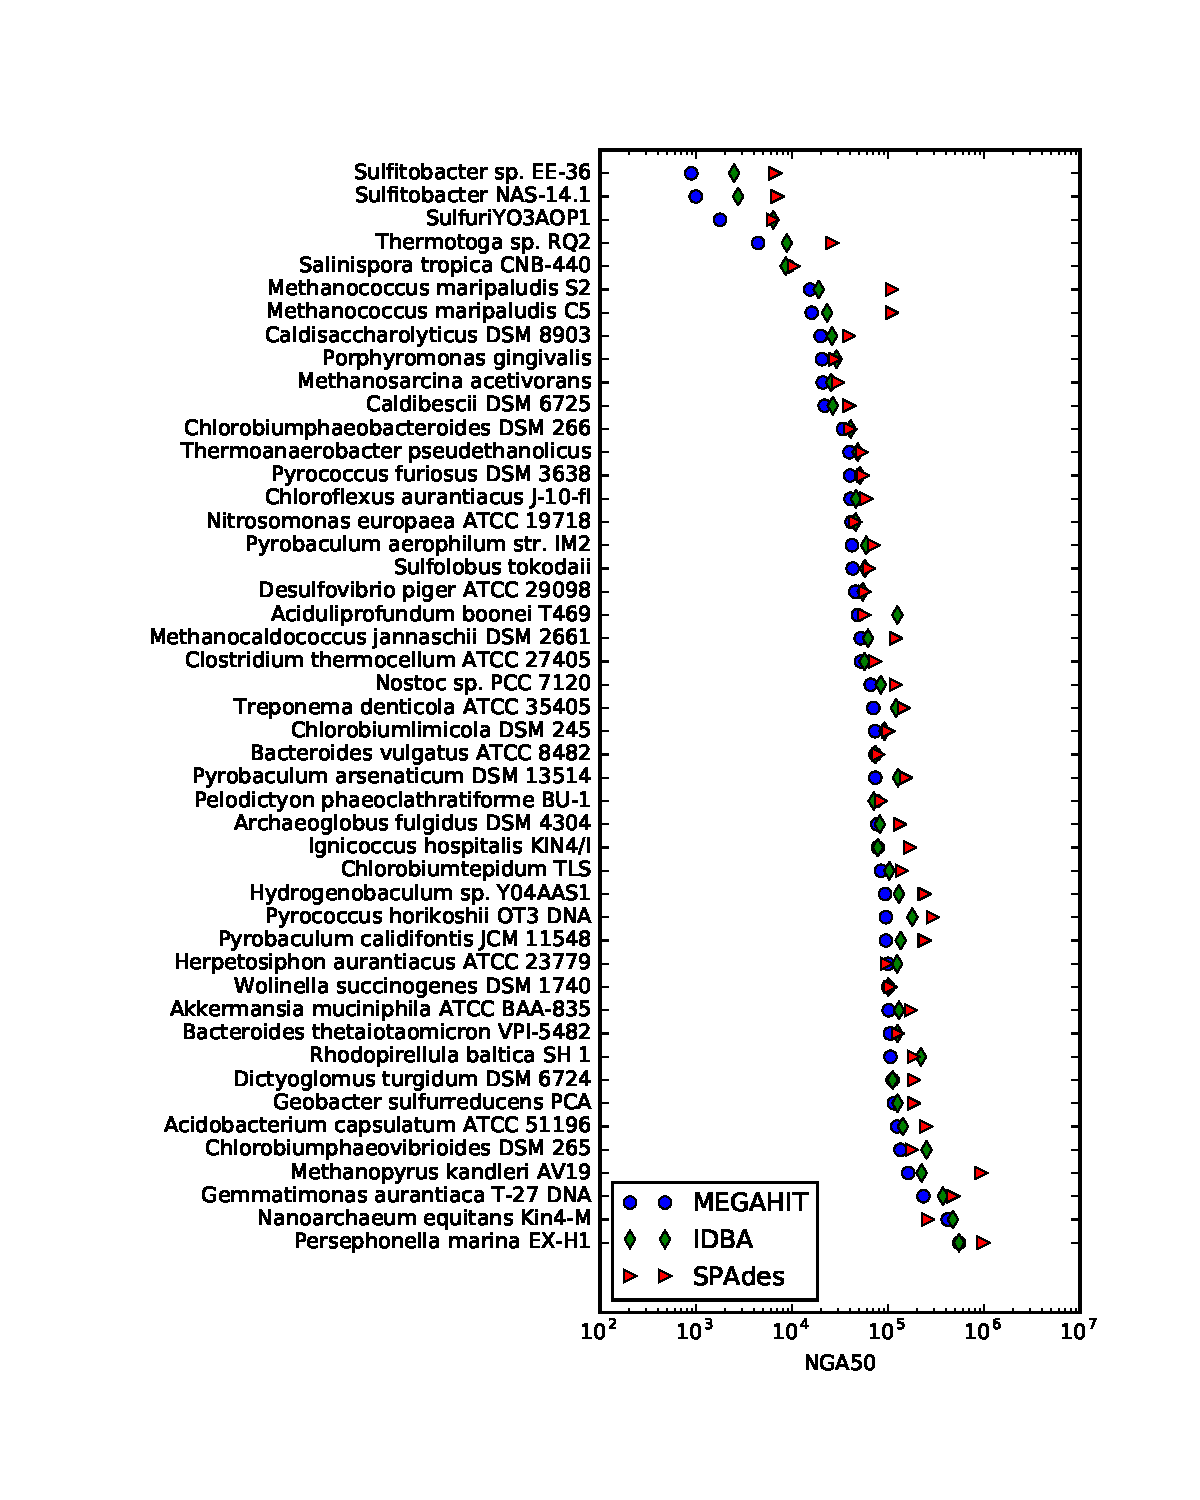
\includegraphics[width=0.9\textwidth]{nga50.pdf}  
\caption{NGA50 by genome and assembler.}
\label{fig:nga50}
\end{figure}



\end{document}

